\FloatBarrier

\begin{figure}[h!]
	\centering
	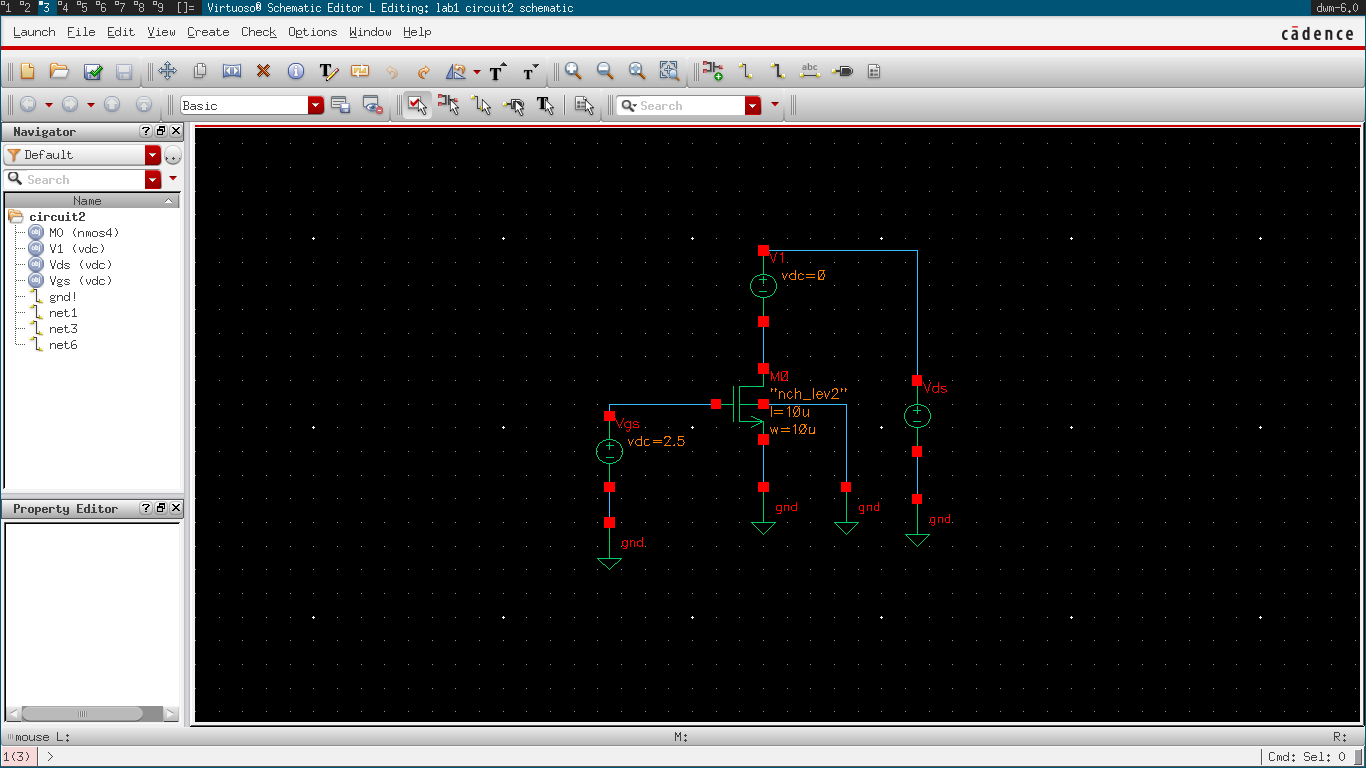
\includegraphics[scale=0.75]{../images/circuit2.PNG}
	\caption{Circuit for Simulation 2}
	\label{fig:circuit2}
\end{figure}

\FloatBarrier

The $I_{D}$ versus $V_{DS}$ characteristics of the n-channel MOSFET are analyzed.
For MOSFETs with channel-length modulation, $r_{o} = \frac{1}{\lambda I_{D}'}$ by definition, where $I_{D}' = \frac{k_{n}}{2} V_{ov}^2$ is the saturation current without channel-length modulation effects.
Here, $V_{ov}$ is the transistor's overdrive voltage, and $k_{n}$ is the MOSFET's transconductance parameter.
The small-signal drain-to-source conductance $g_{ds}$ is to be defined as $g_{ds} = \frac{1}{r_{o}} = \lambda I_{D}'$.
However, $I_{D}'$ is difficult to acquire from realistic simulations. \\

To a first-order approximation, $I_{D} = \frac{k_{n}}{2} V_{ov}^2 ( 1 + \lambda V_{DS} ) = I_{D}' ( 1 + \lambda V_{DS} )$ in saturation mode.
So, $\frac{ \partial I_{D} }{ \partial V_{DS} } = \lambda I_{D}' = g_{ds}$.
Thus, by analyzing the derivative of $I_{D}$ with respect to $V_{DS}$ at a particular value of $V_{DS}$, $g_{ds}$ can be determined from simulation.

First, a simulation is run with $V_{GS} = 0$\si{\volt}.

% TODO Take derivative of ids instead of id in image
% TODO Include source current and show that it is 0 in the image

\FloatBarrier

\begin{figure}[h!]
	\centering
	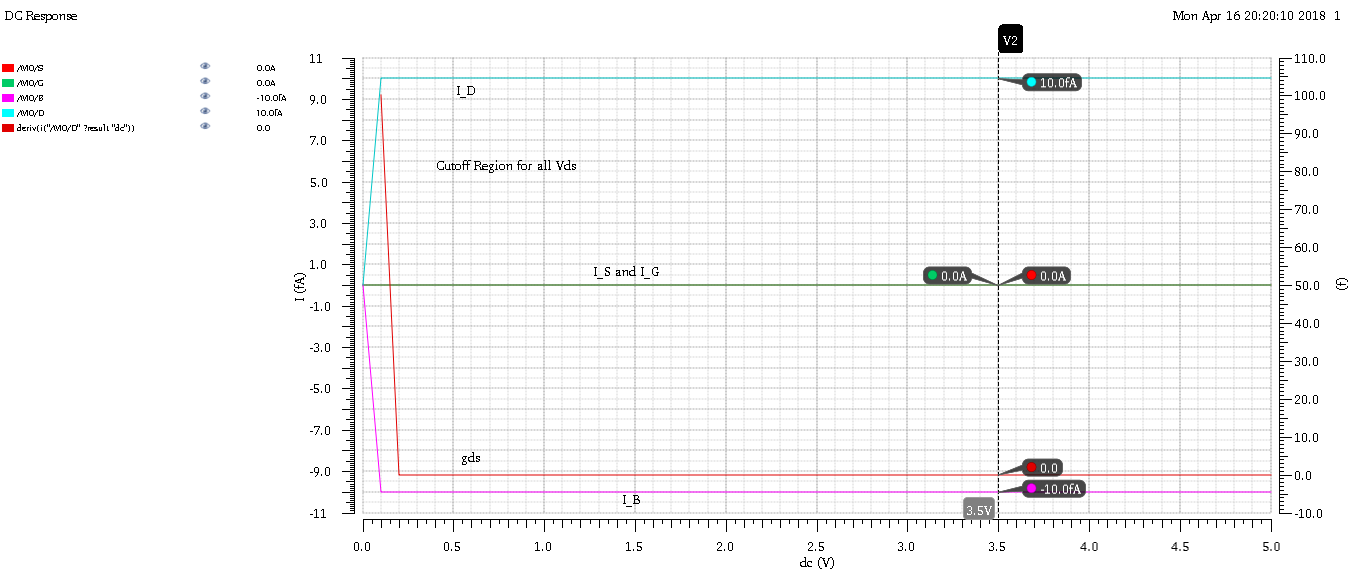
\includegraphics[scale=0.75]{../images/id_vs_vds_vgs_is_0.PNG}
	\caption{NMOS $I_{D}$ versus $V_{DS}$ when $V_{GS} = 0$\si{\volt}}
	\label{fig:id_vs_vds_vgs_is_0}
\end{figure}

\FloatBarrier

Here, $I_{S} = 0$ and $I_{D} = -I_{B} \neq 0$.
Because the transistor is in cutoff mode, no channel between the source and drain forms.
However, the drain's doped n-region forms a pn-junction with the p-type body of the NMOS.
Thermally-generated carriers in the depletion layer become accelerated by the potential difference of the junction's depletion layer.
Thus, a "leakage" current occurs from the drain to the body.
As the drain voltage increases, thermally-generated carriers become accelerated by a larger potential difference, thereby increasing the current.
This relationship can be somewhat accurately modeled by the ideal (or Shockley) diode equation:

\begin{equation}
	\label{eq:shockley_diode}
	I_{DB} = I_{S} ( e^{ \frac{ V_{DB} }{ V_{T} } } - 1 )
\end{equation}

Here, $I_{DB}$ is the current that flows from the drain to the body of the MOSFET.
$I_{S}$ is the reverse saturation current, which is approximately $10$\si{\femto\ampere}.
$V_{DB}$ is the voltage between the drain and the body.
$V_{T} = \frac{ k_{B} T }{ q }$ is the diode's thermal voltage.
For $V_{DB} << -V_{T}$, $I_{DB} \approx -I_{S}$, which explains why the curve is constant for large $V_{DS}$.
Note that $V_{DS} = V_{D} - V_{S} = V_{D} - V_{B} = V_{DB}$. \\

The definition of $g_{ds}$ requires that the transistor be in saturation.
However, if a small signal is to be applied at the MOSFET's gate, one would expect $g_{ds} = 0$ since the channel cannot conduct any current.
Plotting $\frac{ \partial I_{D} }{ \partial V_{DS} }$, labeled $g_{ds}$ in figure (\ref{fig:id_vs_vds_vgs_is_0}), $g_{ds} = 0$ at $V_{DS} = 3.5$\si{\volt}, the particular voltage of interest, consistent with intuition. \\

$V_{GS}$ is now increased to $2.5\si{\volt}$.
In the triode region, $I_{D}$ depends on $-V_{DS}^{2}$ because $I_{D} = k_{n} ( V_{ov} - 0.5 V_{DS} ) V_{DS}$.
So, $\frac{ \partial I_{D} }{ \partial V_{DS} }$ depends linearly on $-V_{DS}$.
In the saturation region, $\frac{ \partial I_{D} }{ \partial V_{DS} }$ is constant with $V_{DS}$.
Therefore, the transition point between a linear curve and a constant curve marks the transition from saturation to triode, whose intervals are labeled in figure (\ref{fig:id_vs_vds_vgs_is_2_5}).

\FloatBarrier

\begin{figure}[h!]
	\centering
	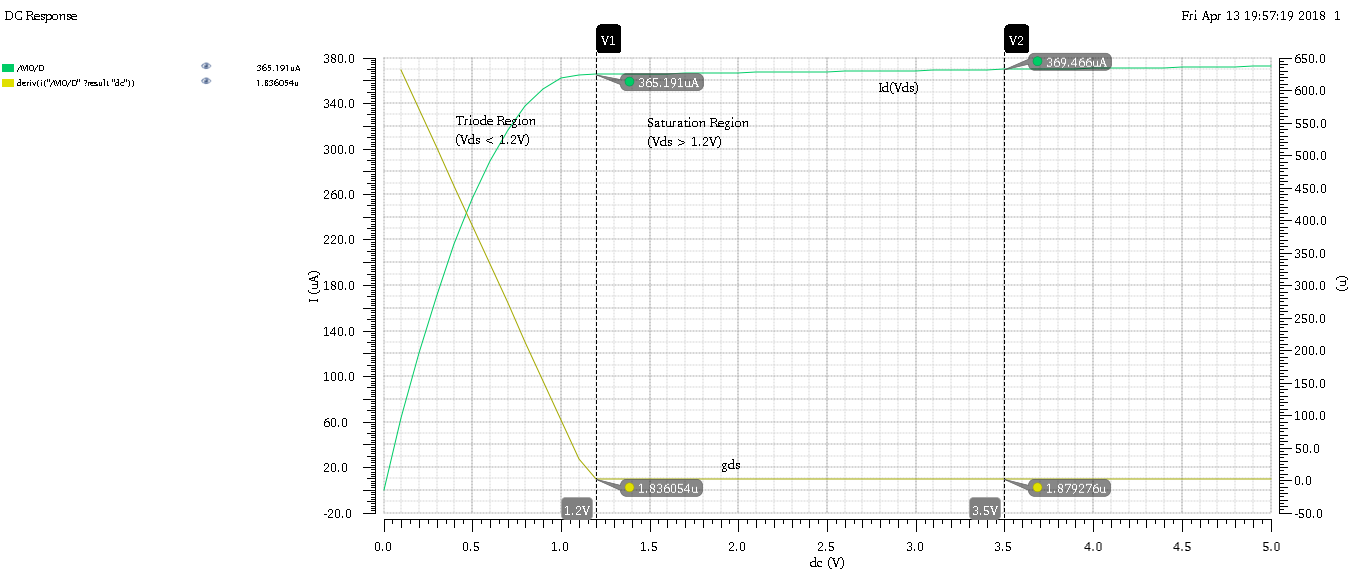
\includegraphics[scale=0.75]{../images/id_vs_vds_vgs_is_2_5.PNG}
	\caption{NMOS $I_{D}$ versus $V_{DS}$ when $V_{GS} = 2.5$\si{\volt}}
	\label{fig:id_vs_vds_vgs_is_2_5}
\end{figure}

\FloatBarrier

Here, $g_{ds}$ can be properly evaluated since the transistor is analyzed at $V_{DS} = 3.5$\si{\volt}, which occurs in the saturation region.

\FloatBarrier

\begin{figure}[h!]
	\centering
	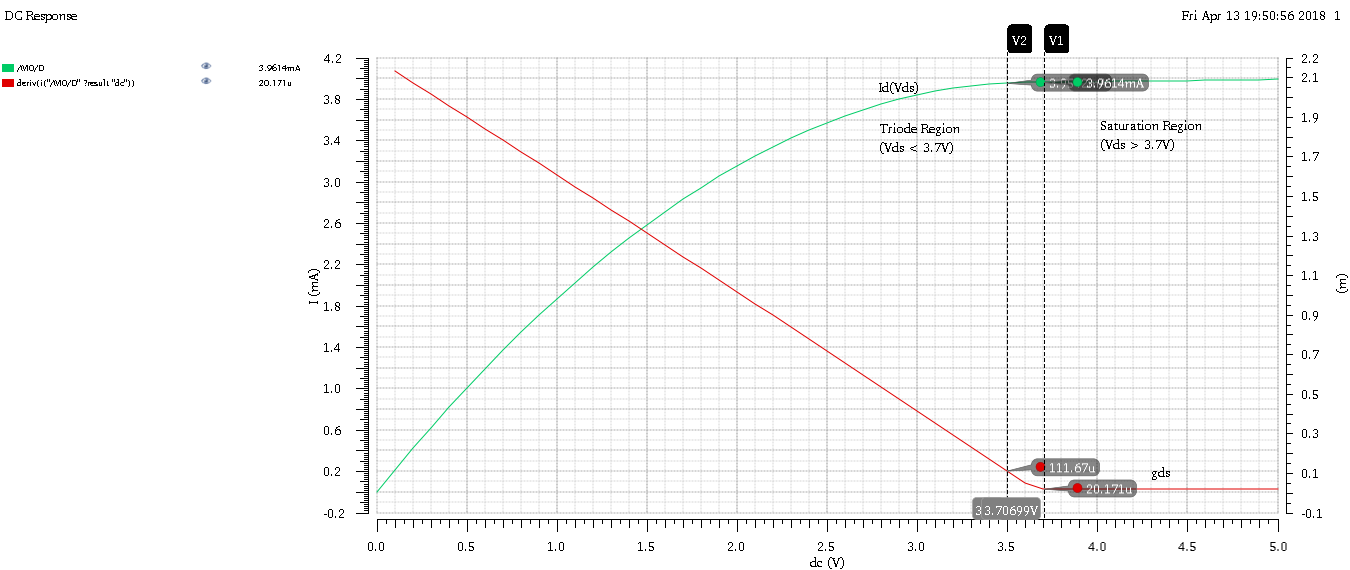
\includegraphics[scale=0.75]{../images/id_vs_vds_vgs_is_5.PNG}
	\caption{NMOS $I_{D}$ versus $V_{DS}$ when $V_{GS} = 5.0$\si{\volt}}
	\label{fig:id_vs_vds_vgs_is_5}
\end{figure}

\FloatBarrier

The simulation results for $V_{GS} = 5.0$\si{\volt} are shown in figure (\ref{fig:id_vs_vds_vgs_is_5}).
The transistor operates in the triode region at $V_{DS} = 3.5$\si{\volt}, but the same definition is applied nonetheless.
The final results are tabulated in table (\ref{tab:sim2_results}).

\FloatBarrier

\begin{table}[h!]
	\centering
	\caption{Simulation 2 Results}
	\label{tab:sim2_results}
	\csvautotabular{../tables/sim2_results.csv}
\end{table}

\FloatBarrier

% Determine lambda
